\documentclass{article}
\usepackage{amsmath}
\usepackage{bm}
\usepackage[UTF8]{ctex}
\usepackage{wrapfig}
\usepackage{hep}
\usepackage{simplewick}
\usepackage{caption}
\usepackage{graphicx}
\usepackage{geometry}
\usepackage{tikz}
\usepackage{color}
\usepackage{graphicx}
\usepackage{subfig}
\usepackage{xcolor}
\usepackage{hep}
\usepackage{physics}
\usepackage{listings}
\usepackage{animate}

\geometry{a4paper,left=2cm,right=2cm,top=2cm,bottom=2cm}

\newcommand{\mk}{\mathbf{k}}
\newcommand{\mR}{\mathbf{R}}

\lstset{
 columns=fixed,       
 numbers=left,                                        % 在左侧显示行号
 numberstyle=\tiny\color{gray},                       % 设定行号格式
 frame=none,                                          % 不显示背景边框
 backgroundcolor=\color[RGB]{245,245,244},            % 设定背景颜色
 keywordstyle=\color[RGB]{40,40,255},                 % 设定关键字颜色
 numberstyle=\footnotesize\color{darkgray},           
 commentstyle=\it\color[RGB]{0,96,96},                % 设置代码注释的格式
 stringstyle=\rmfamily\slshape\color[RGB]{128,0,0},   % 设置字符串格式
 showstringspaces=false,                              % 不显示字符串中的空格
 language=python,                                        % 设置语言
}

\begin{document}
\title{非厄米系统的边缘态和拓扑不变量}
\maketitle
\section{简介}
拓扑材料具有抗扰动的鲁棒边界态。根据体-边界对应原理,边界状态的存在由体拓扑不变量决定,在能带理论框架下,用布洛赫哈密顿量定义了体拓扑不变量。这个哈密顿通常被假设成厄米的。在许多物理系统里,非厄米哈密顿更为合适。例如,它们被广泛用于描述开放系统,具有增益和损失的波系统(例如,光子和声学),以及电子-电子相互作用或无序将非厄米特自能引入准粒子有效哈密顿量的固体系统。由于这些物理动机,最近有越来越多的努力,理论和实验,研究非厄米顿拓扑现象。

其中一个关键问题是非厄米系统中体边界对应的形式。近年来,在一维(1D)模型上的数值结果表明,开边界谱与周期边界谱有很大的不同,这似乎表明了体-边界对应的完全分解。鉴于这种分解,一种可能的情况是拓扑边缘状态依赖于所有的样本细节,没有任何一般规则告诉它们的存在或消失。在这里,我们提出以下问题:是否存在广义的体边界对应?是否存在与拓扑边缘态对应的体拓扑不变量?在本文中得到了肯定的答复。

我们从一维模型开始。有趣的是,开链的所有本征态都局限在边界附近(称为“非厄米趋肤效应”),而不是厄米特情况下的扩展布洛赫波。在最简单的情况下,这种效应可以用一个假想的规范场来理解。我们证明了非厄米趋肤效应在建立“非布洛赫体-边界对应”时具有显著的结果,其中拓扑边模由“非bloch拓扑不变量”决定。

以前的非厄米特拓扑不变量是用布洛赫哈密顿量来表述的。本征态的非布洛赫波特性(非厄米趋肤效应)未被触及;因此,拓扑边模的数量一般与这些拓扑不变量无关。针对非厄米特蒙皮效应,引入非布洛赫拓扑不变量,忠实地确定拓扑边模数。它体现了非厄米系统的非布洛赫体-边界对应。
\section{模型}
非厄米Su-Schrieffer-Heeger(SSH)模型如图1所示
\begin{figure}[h]
    \centering
    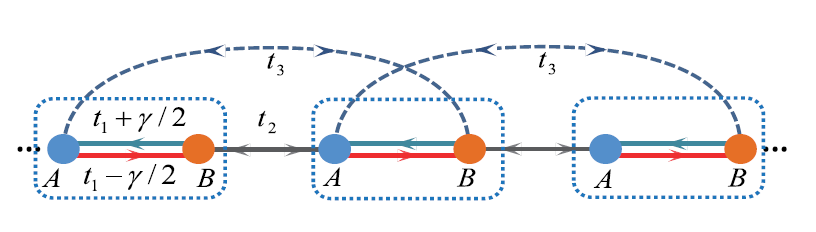
\includegraphics[width=4in]{fig1.png}
    \caption{非厄米SSH模型。框内的点代表单位原胞}
\end{figure}
格点空间的哈密顿形式为
\begin{equation}
    H=(t_1+\frac{\gamma}{2})c_{A,n}^\dagger c_{B,n}+(t_1-\frac{\gamma}{2})c_{B,n}^\dagger c_{A,n}^\dagger+t_2c_{B,n}^\dagger c_{A,n+1}+t_2c_{A,n+1}^\dagger c_{B,n}+t_3 c_{A,n}^\dagger c_{B,n+1}+t_3c_{B,n+1}^\dagger c_{A,n}
\end{equation}
\begin{equation}
    H=\begin{pmatrix}
        0&t_1+\gamma/2\\
        t_1-\gamma/2&0&t_2\\
        &t_2&0&t_1+\gamma/2\\
        &&\cdots&\cdots&\cdots
    \end{pmatrix}
\end{equation}
利用傅里叶变换:
\begin{equation*}
    \begin{split}
        c_{A,n}&=\frac{1}{\sqrt{Na}}\sum_{k}e^{i\mk\cdot\mR_n}c_{A,k}\\
        c_{B,n}&=\frac{1}{\sqrt{Na}}\sum_{k}e^{i\mk\cdot\mR_n}c_{B,k}
    \end{split}
\end{equation*}
得到
\begin{equation}
    \begin{split}
        H&=(t_1+\frac{\gamma}{2})\sum_{k}c_{A,k}^\dagger c_{B,k}+(t_1-\frac{\gamma}{2})\sum_{k}c_{B,k}^\dagger c_{A,k}+t_2\sum_{k}e^{ika}c_{B,k}^\dagger c_{A,k}+t_2\sum_{k}e^{-ika}c_{A,k}^\dagger c_{B,k}\\
        &+t_3\sum_{k}e^{ika}c_{A,k}^\dagger c_{B,k}+t_3\sum_{k}e^{-ika}c_{B,k}^\dagger c_{A,k}
    \end{split}
\end{equation}
写成BdG形式:
\begin{equation}
    H=\sum_{k}\begin{pmatrix}
        c_{A,k}^\dagger&c_{B,k}^\dagger
    \end{pmatrix}\begin{pmatrix}
        0&(t_1+\frac{\gamma}{2})+t_2e^{-ika}+t_3e^{ika}\\
        (t_1-\frac{\gamma}{2})+t_2e^{ika}+t_3e^{-ika}
    \end{pmatrix}\begin{pmatrix}
        c_{A,k}\\
        c_{B,k}
    \end{pmatrix}
\end{equation}
布洛赫哈密顿为
\begin{equation}
    H(k)=d_x\sigma_x+(d_y+i\frac{\gamma}{2})\sigma_y
\end{equation}
其中$d_x=t_1+(t_2+t_3)\cos ka,d_y=(t_2-t_3)\sin ka$。$\sigma_{x,y}$是泡利矩阵。在一些文章中$\sigma_y$被替代成$\sigma_z$;因此,物理解释不是SSH。这个模型有一个子格对称性
\begin{equation}
    \sigma_z^{-1}H(k)\sigma_{z}-H(k)
\end{equation}
这保证了本征值成对出现$(E,-E)$:
\begin{equation}
    \begin{split}
        H(k)|u(k)\rangle&=E(k)|u(k)\rangle\\
        H(k)\sigma_z|u(k)\rangle&=-\sigma_z H(k)|u(k)\rangle=-E\sigma_z|u(k)\rangle
    \end{split}
\end{equation}
所以我们得到:
\begin{equation}
    E_{\pm}=\pm\sqrt{d_x^2+(d_y+i\frac{\gamma}{2})^2}
\end{equation}
分别对应这两个能量。为了简单起见,首先我们令$t_3=0$. 令$E_{\pm}(k)=0$得到
\begin{equation}
    \begin{cases}
        &d_x^2+d_y^2-\frac{\gamma^2}{4}=0\\
        &d_y\frac{\gamma}{2}=0
    \end{cases}\Longrightarrow \begin{cases}
        &d_x=\pm\frac{\gamma}{2}\\
        &d_y=0
    \end{cases}
\end{equation}
能隙正在ep点处关闭$(d_x,d_y)=(\pm\gamma/2,0)$,这要求:
\begin{equation}
    \begin{cases}
        &t_1+t_2\cos ka=\pm\frac{\gamma}{2}\\
        &t_2\sin ka=0
    \end{cases}\Longrightarrow\begin{cases}
        t_1=-t_2\pm\frac{\gamma}{2}\quad&(k=0)\\
        t_1=t_2\pm\frac{\gamma}{2}\quad&(k=0)
    \end{cases}
\end{equation}
开边界谱与周期边界谱有明显的不同,这可以在开链的实空间哈密顿量的数值谱中看到。
\begin{figure}[htbp]
\centering
\begin{minipage}[t]{0.3\textwidth}
\centering
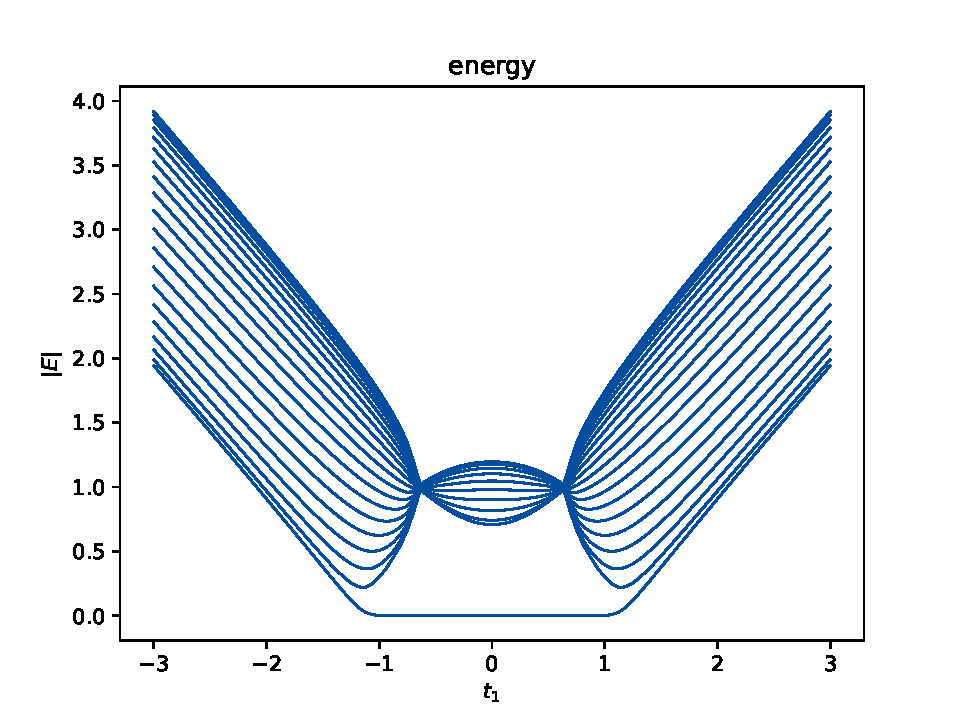
\includegraphics[width=2in]{Figure_1.pdf}
\caption{能量}
\end{minipage}
\begin{minipage}[t]{0.3\textwidth}
\centering
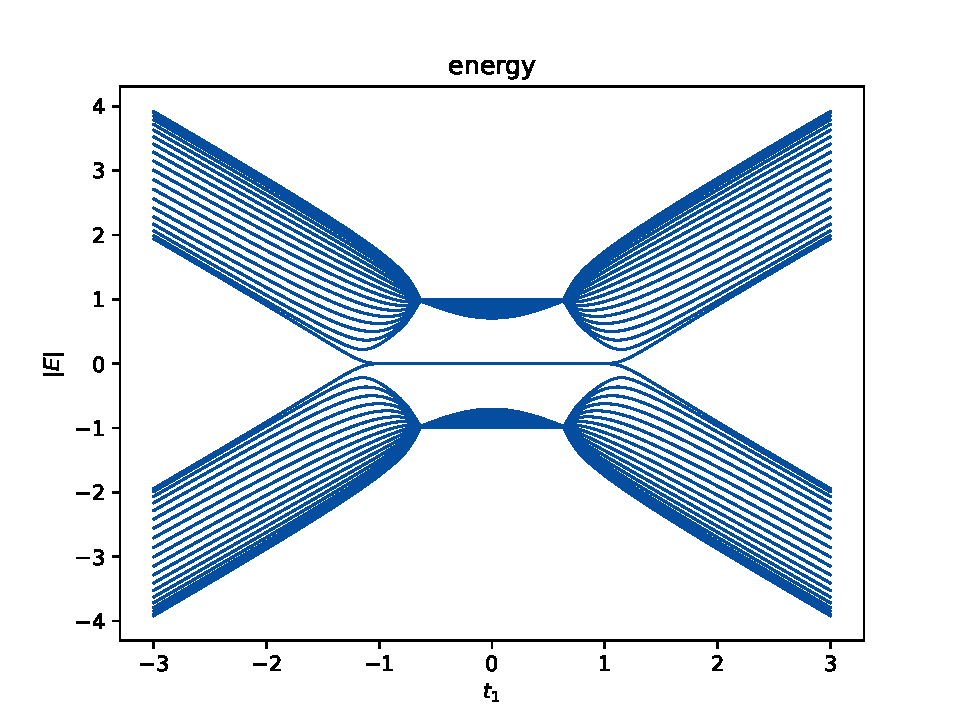
\includegraphics[width=2in]{Figure_2.pdf}
\caption{实部}
\end{minipage}
\begin{minipage}[t]{0.3\textwidth}
    \centering
    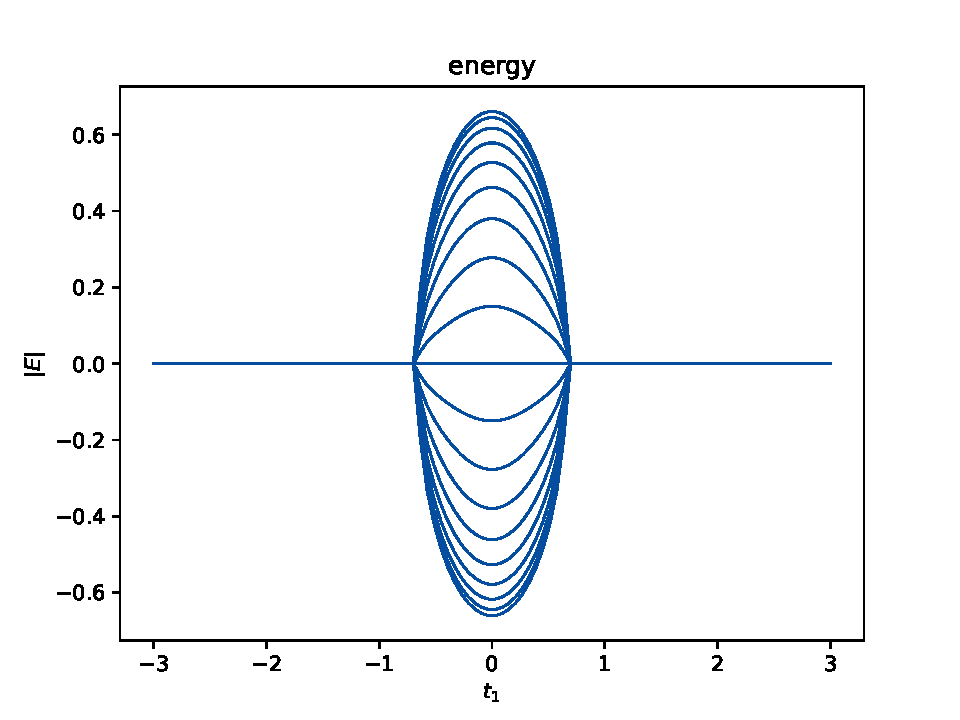
\includegraphics[width=2in]{Figure_3.pdf}
    \caption{虚部}
    \end{minipage}
\end{figure}
\begin{lstlisting}
    import matplotlib.pyplot as plt
    import numpy as np
    t2=1
    gamma=4/3
    num=40
    eiva=[]
    h=np.zeros([num,num])
    #定义一个返回第n带的能谱函数
    def eiv(t1,n):
        for i in range(0,num,2):
            h[i][i+1]=t1+gamma/2
            h[i+1][i]=t1-gamma/2
        for i in range (1,num-1,2):
            h[i][i+1]=t2
            h[i+1][i]=t2
        e,v=np.linalg.eig(h)
        e=np.sort(abs(e))
        return e[n]
    t1=np.linspace(-3,3,100)
    for n in range(0,num):
        energy=[eiv(x,n) for x in t1]
        plt.title("energy") 
        plt.xlabel("$t_1$") 
        plt.ylabel("$|E|$") 
        plt.plot(t1,energy,c="#054E9F",linewidth=1)
    plt.show()
\end{lstlisting}
零模对扰动的robust表明了它们的拓扑起源。相变点位于$t1\approx 1.20$,从$H(k)$的能谱上看,这是一个非常不起眼的点,能谱在这里发生闭合,并且$E_\pm(k)\neq0$。$H(k)$的拓扑并不能决定零模,这与厄米情况相悖。
\section{截断}
开链波函数定义成
\begin{equation}
    |\psi\rangle=(\psi_{1,A},\psi_{1,B},\psi_{2,A},\psi_{2,B},\cdot,\psi_{L,A},\psi_{L,B})^T
\end{equation}
做一个截断,考虑$t_3=0$的情况。实空间本征方程可以变换为
\begin{equation}
    H|\psi\rangle=E|\psi\rangle\Rightarrow \bar{H}|\bar{\psi}\rangle=E|\bar{\psi}\rangle
\end{equation}
其中:
\begin{equation}
    |\bar{\psi}\rangle=S^{-1}|\psi\rangle,\quad \bar{H}=S^{-1}HS
\end{equation}
令$S=diag\{1,r,r,r^2,r^2,\cdots,r^{L-1},r^{L-1},r^L\}$
\begin{equation}
    \bar{H}=S^{-1}HS=diag\{1,r^{-1},r^{-1},r^{-2},r^{-2},\cdots,r^{-L+1},r^{-L+1},r^{-L}\}Hdiag\{1,r,r,r^2,r^2,\cdots,r^{L-1},r^{L-1},r^L\}
\end{equation}
\begin{equation}
    \begin{split}
        \bar{H}&=\begin{pmatrix}
            1\\
            &r^{-1}\\
            &&r^{-1}\\
            &&&\vdots\\
            &&&&r^{-L+1}\\
            &&&&&r^{-L+1}\\
            &&&&&&r^L
        \end{pmatrix}\begin{pmatrix}
            0&t_1+\frac{\gamma}{2}\\
            t_1-\frac{\gamma}{2}&0&t_2\\
            &t_2&0&t_1+\frac{\gamma}{2}\\
            &&\cdots&\cdots&\cdots
        \end{pmatrix}
            \begin{pmatrix}
            1\\
            &r^{1}\\
            &&r^{1}\\
            &&&\vdots\\
            &&&&r^{L-1}\\
            &&&&&r^{L-1}\\
            &&&&&&r^L
        \end{pmatrix}\\
        &=\begin{pmatrix}
            0&r(t_1+\frac{\gamma}{2})\\
            r^{-1}(t_1-\frac{\gamma}{2})&0&t2\\
            &t2&0&\cdots\\
            &&\cdots&\cdots&r(t_1+\frac{\gamma}{2})\\
            &&&r^{-1}(t_1-\frac{\gamma}{2})&0
        \end{pmatrix}
    \end{split}
\end{equation}
令$r=\sqrt{|\frac{t_1-\frac{\gamma}{2}}{t_1+\frac{\gamma}{2}}|}$得到
\begin{equation}
    \begin{split}
        r(t_1+\frac{\gamma}{2})&=\sqrt{|t_1-\frac{\gamma}{2}||t_1+\frac{\gamma}{2}|}\\
        r^{-1}(t_1-\frac{\gamma}{2})&=\sqrt{|t_1+\frac{\gamma}{2}||t_1-\frac{\gamma}{2}|}
    \end{split}
\end{equation}
对于$|t_1|>|\frac{\gamma}{2}|$的情况,晶格内部和晶格之间的Hopping为
\begin{equation}
    \bar{t}_1=\sqrt{(t_1-\gamma/2)(t_1+\gamma/2)},\quad \bar{t}_2=t_2
\end{equation}
$k$空间的哈密顿表达式为
\begin{equation}
    \bar{H}(k)=(\bar{t}_1+\bar{t}_2\cos ka)\sigma_x+\bar{t}_2\sin ka\sigma_y
\end{equation}
相变点发生在$\bar{t}_1=\bar{t}_2(ka=\pi)$,也就是说
\begin{equation}
    \sqrt{(t_1-\gamma/2)(t_1+\gamma/2)}=t_2\Rightarrow t_1^2-\gamma^2/4=t_2^2\Rightarrow t_1=\pm\sqrt{t_2^2+\gamma^2/4}
\end{equation}
对于上图给的能谱图,上式给出相变点$t_1=\pm 1.2$。值得注意,任何基于$H(k)$的拓扑不变量仅仅在能隙闭合的点$t_1=\pm t_2\pm\gamma/2$发生跳跃。

这里先分析一下$r>1$的条件
\begin{equation}
    r=\sqrt{|\frac{t_1-\gamma/2}{t_1+\gamma/2}|}>1\Rightarrow|\frac{t_1-\gamma/2}{t_1+\gamma/2}|>1\Rightarrow\frac{|t_1-\gamma/2|-|t_1+\gamma/2|}{|t_1+\gamma/2|}>0
\end{equation}
\begin{equation}
    \begin{cases}
        t_1<0\\
        t_1>-\gamma/2
    \end{cases},\quad\begin{cases}
        t_1<0\\
        t_1<-\gamma/2
    \end{cases}
\end{equation}
考虑到$|t_1|>|\gamma/2|$,第一个解要舍去。

厄米算符$\bar{H}$的体本征态$|\bar{\psi}_l\rangle$是扩展的;因此$H$的本征态$|\psi_l\rangle=S|\bar{\psi}_l\rangle$是指数化局域在链的边界的$(\gamma\neq 0)$
\begin{equation}
    \begin{pmatrix}
        \psi_{1,A}\\
        \psi_{1,B}\\
        \psi_{2,A}\\
        \psi_{2,B}\\
        \cdots\\
        \psi_{L,A}\\
        \psi_{L,B}
    \end{pmatrix}=\begin{pmatrix}
        \bar{\psi}_{1,A}\\
        r\bar{\psi}_{1,B}\\
        r\bar{\psi}_{2,A}\\
        r^2\bar{\psi}_{2,B}\\
        \cdots\\
        r^{L-1}\bar{\psi}_{L,A}\\
        r^{L}\bar{\psi}_{L,B}
    \end{pmatrix}
\end{equation}
$|\bar{\psi}_{l,s}\rangle(l=1,\cdots,L;s=A,B)$是$\bar{H}$的本征态,$\bar{H}$又是厄米的,所以$|\bar{\psi}_{l,s}\rangle$有布洛赫因子$e^{ik\cdot R}$。对于一维SSH模型,$R=na$,$a$是原胞长度。对于截断的SSH模型来说,波函数可以写成
\begin{equation}
    \begin{pmatrix}
        \bar{\psi}_{1,A}\\
        \bar{\psi}_{1,B}\\
        \bar{\psi}_{2,A}\\
        \bar{\psi}_{2,B}\\
        \cdots\\
        \bar{\psi}_{L,A}\\
        \bar{\psi}_{L,B}
    \end{pmatrix}=\begin{pmatrix}
        u_{1,A}\\
        e^{ika}u_{1,B}\\
        e^{ika}u_{2,A}\\
        e^{ik2a}u_{2,B}\\
        \cdots\\
        e^{ik(L-1)a}u_{L,A}\\
        e^{ikLa}u_{L,B}
    \end{pmatrix}
\end{equation}
所以对于开边界$\psi_l$来说,布洛赫因子$e^{ika}$替换成$re^{ika}$是合理的。
\begin{equation}
    re^{ika}=e^{ika+lnr}=e^{i(ka-i\ln r)}
\end{equation}
波矢量获得了一个虚部:$k\rightarrow k-i\ln r$. 尽管这个直观图像是基于截断解,但是我们相信本征态的指数衰减行为是非厄米能带的一般性质。

\section{一般解}
直观的截断解有限制,例如在$t_3\neq 0$时不适用。这里我们通过更一般的方式重新推导了这个解。为了简单起见,我们仍然令$t_3=0$. 实空间的本征方程为
\begin{equation}
    \begin{split}
        t_2\psi_{n-1,B}+(t_1+\gamma/2)\psi_{n,B}&=E\psi_{n,A}\\
        (t_1-\gamma/2)\psi_{n,A}+t_2\psi_{n+1,A}&=E\psi_{n,B}
    \end{split}
\end{equation}
我们从拟设解出发
\begin{equation}
    \begin{pmatrix}
        \psi_{1,A}\\
        \psi_{1,B}\\
        \cdots\\
        \psi_{L,A}\\
        \psi_{L,B}
    \end{pmatrix}=|\psi\rangle=\sum_{j}|\phi^{(j)}\rangle=\sum_{j}\begin{pmatrix}
        \phi_{1,A}^{(j)}\\
        \phi_{1,B}^{(j)}\\
        \cdots\\
        \phi_{L,A}^{(j)}\\
        \phi_{L,B}^{(j)}
    \end{pmatrix}
\end{equation}
其中每一个$|\phi^{(j)}\rangle$有指数形式:
\begin{equation}
    \begin{pmatrix}
        \phi_{n,A}\\
        \phi_{n,B}
    \end{pmatrix}=\beta^n\begin{pmatrix}
        \phi_A\\
        \phi_B
    \end{pmatrix}
\end{equation}
带入SSH模型的实空间本征方程得到
\begin{equation}
    \begin{split}
        \left[(t_1+\gamma/2)+t_2\beta^{-1}\right]\phi_B&=E\phi_A\\
        \left[(t_1-\gamma/2)+t_2\beta\right]\phi_A&=E\phi_B
    \end{split}
\end{equation}
因此我们有
\begin{equation}
    \left[\left(t_1-\frac{\gamma}{2}\right)+t_2\beta\right]\left[\left(t_1+\frac{\gamma}{2}\right)+t_2\beta^{-1}\right]=E^2
\end{equation}
求解一下这个方程
\begin{equation}\label{beta-eq}
    (t_1+\frac{\gamma}{2})t_2\beta^2+(t_1^2-\frac{\gamma^2}{4}+t_2^2)\beta+(t_1-\frac{\gamma}{2})t_2-E^2\beta=0
\end{equation}
得到:
\begin{equation}
    \begin{split}
        \beta_1(E)=\frac{E^2+\gamma^2/4-t_1^2-t_2^2+\sqrt{(E^2+\gamma^2/4-t_1^2-t_2^2)^2-4t_2^2(t_1^2-\gamma^2/4)}}{2t_2(t_1+\gamma/2)}\\
        \beta_2(E)=\frac{E^2+\gamma^2/4-t_1^2-t_2^2-\sqrt{(E^2+\gamma^2/4-t_1^2-t_2^2)^2-4t_2^2(t_1^2-\gamma^2/4)}}{2t_2(t_1+\gamma/2)}
    \end{split}
\end{equation}
取$E\to 0$极限得到
\begin{equation}
    \begin{split}
        \beta_1&=-\frac{t_1^2+t_2^2-\gamma^2/4+|t_1^2-t_2^2-\gamma^2/4|}{2t_2(t_1+\gamma/2)}\\
        \beta_2&=-\frac{t_1^2+t_2^2-\gamma^2/4-|t_1^2-t_2^2-\gamma^2/4|}{2t_2(t_1+\gamma/2)}
    \end{split}
\end{equation}
对于$|t_1|>\sqrt{t_2^2+\gamma^2/4}$有
\begin{equation}
    \beta_1=-\frac{t_1-\gamma/2}{t_2},\quad \beta_2=-\frac{t_2}{t_1+\gamma/2}
\end{equation}
对于$|t_1|<\sqrt{t_2^2+\gamma^2/4}$有
\begin{equation}
    \beta_1=-\frac{t_2}{t_1+\gamma/2},\quad \beta_2=-\frac{t_1-\gamma/2}{t_2}
\end{equation}
可以看到这两个解分别对应$\phi_A=0$和$\phi_B=0$

补上指标$j$后,我们有
\begin{equation}
    \begin{split}
        \phi_A^{(j)}&=\frac{E}{(t_1-\gamma/2)+t_2\beta_j}\phi_B^{(j)}\\
        \phi_B^{(j)}&=\frac{E}{(t_1+\gamma/2)+t_2\beta_j^{-1}}\phi_B^{(j)}
    \end{split}
\end{equation}
这两个方程等价。通解可以写成线性组合形式
\begin{equation}
    \begin{pmatrix}
        \psi_{n,A}\\
        \psi_{n,B}
    \end{pmatrix}=\begin{pmatrix}
        \phi_{n,A}^{(1)}\\
        \phi_{n,B}^{(1)}
    \end{pmatrix}+\begin{pmatrix}
        \phi_{n,A}^{(2)}\\
        \phi_{n,B}^{(2)}
    \end{pmatrix}=\beta^{n}_1\begin{pmatrix}
        \phi_{A}^{(1)}\\
        \phi_{B}^{(1)}
    \end{pmatrix}+\beta_2^{n}\begin{pmatrix}
        \phi_{A}^{(2)}\\
        \phi_{B}^{(2)}
    \end{pmatrix}
\end{equation}
满足边界条件
\begin{equation}
    \begin{split}
        \left(t_1+\frac{\gamma}{2}\right)\psi_{1,B}-E\psi_{1,A}&=0\\
        \left(t_2-\frac{\gamma}{2}\right)\psi_{L,A}-E\psi_{L,B}&=0
    \end{split}
\end{equation}
把线性组合形式带入上式得到
\begin{equation}
    \begin{split}
        \left(t_1+\frac{\gamma}{2}\right)(\beta_1\phi_B^{(1)}+\beta_2\phi_B^{(2)})-E\left(\beta_1\phi_A^{(1)}+\beta_2\phi_A^{(2)}\right)&=0\\
        \left(t_1-\frac{\gamma}{2}\right)(\beta_1^L\phi_A^{(1)}+\beta_2^L\phi_B^{(2)})-E\left(\beta_1^L\phi_B^{(1)}+\beta_2^L\phi_B^{(2)}\right)&=0
    \end{split}
\end{equation}
带入$\phi_A$和$\phi_B$之间的关系
\begin{equation}
    \begin{split}
        \left(t_1+\frac{\gamma}{2}\right)\left(\beta_1\phi_B^{(1)}+\beta_2\phi_B^{(2)}\right)-E\left(\beta_1\frac{E}{t_1-\frac{\gamma}{2}+t_2\beta_1}\phi_B^{(1)}+\beta_2\frac{E}{t_1-\frac{\gamma}{2}+t_2\beta_2}\phi_B^{(2)}\right)&=0\\
        \left(t_1-\frac{\gamma}{2}\right)\left(\beta_1^L\frac{E}{t_1-\frac{\gamma}{2}+t_2\beta_1}\phi_B^{(1)}+\beta_2^L\frac{E}{t_1-\frac{\gamma}{2}+t_2\beta_2}\phi_B^{(2)}\right)-E\left(\beta_1^L\phi_B^{(1)}+\beta_2^L\phi_B^{(2)}\right)&=0
    \end{split}
\end{equation}
带入$\left[\left(t_1-\frac{\gamma}{2}\right)+t_2\beta\right]\left[\left(t_1+\frac{\gamma}{2}\right)+t_2\beta^{-1}\right]=E^2$
得到
\begin{equation}
    \begin{split}
        &\frac{t_2\beta_1^{L+1}}{t_1-\frac{\gamma}{2}+t_2\beta_1}\phi_B^{(1)}+\frac{t_2\beta_2^{L+1}}{t_1-\frac{\gamma}{2}+t_2\beta_2}\phi_B^{(2)}=0\\
        &t_2\phi_B^{(1)}+t_2\phi_B^{(2)}=0\\
    \end{split}
\end{equation}
化简得到:
\begin{equation}
    \beta_1^{L+1}(t_1-\frac{\gamma}{2}+t_2\beta_2)=\beta_2^{L+1}(t_1-\frac{\gamma}{2}+t_2\beta_1)
\end{equation}
我们关注的是长链的谱,对于体本征态来说必须有$|\beta_1|=|\beta_2|$. 如果不是这样,我们假设$|\beta_1|<|\beta_2|$,我们可以舍去$\beta_1^{L+1}$项,方程变成$\beta=0$或者$t_1-\frac{\gamma}{2}+t_2\beta_1=0$. 由于体带的性质,在有边缘附近的扰动下,$|\beta_1(E)|=|\beta_2(E)|$仍然有效,并且决定了体带的能量。
\begin{figure}[h]
    \centering
    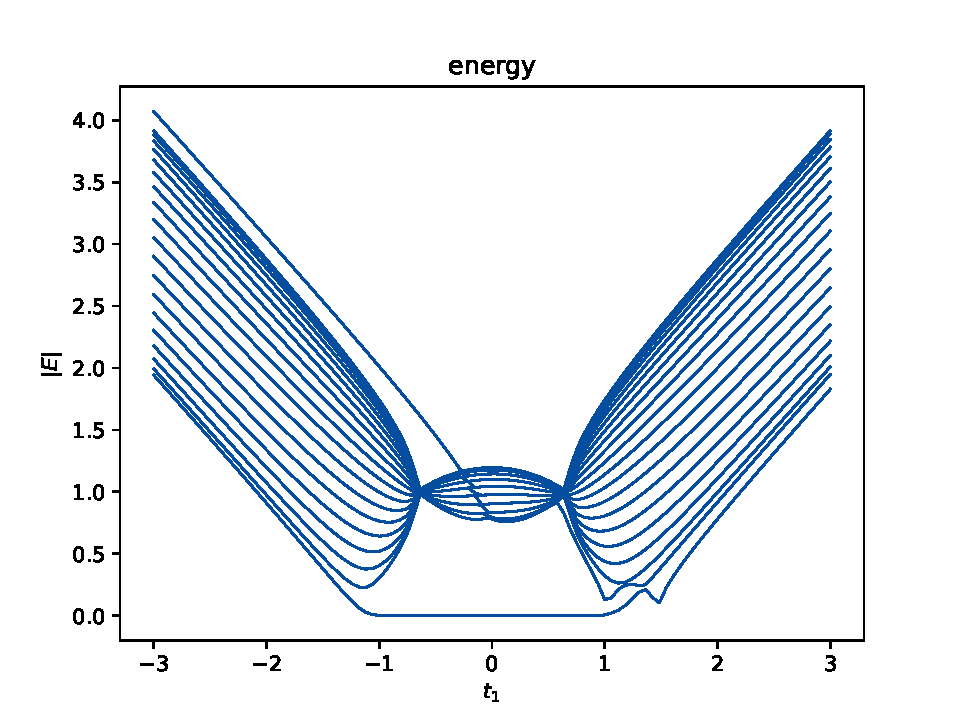
\includegraphics[width=4in]{Figure_4.pdf}
    \caption{在链的最左端加了扰动,变成$t_1-0.8$,这导致了额外的非零模,但是零模并没有被影响}
\end{figure}
\begin{lstlisting}
    import matplotlib.pyplot as plt
    import numpy as np
    t2=1
    gamma=4/3
    num=40
    p=0.1
    t1list=[-3+p*i for i in range(0,int(6/p)+1)]
    eiva=[]
    h=np.zeros([num,num])
    #定义一个返回第n带的能谱函数
    def eiv(t1,n):
        for i in range(0,num,2):
            h[i][i+1]=t1+gamma/2
            h[i+1][i]=t1-gamma/2
        for i in range (1,num-1,2):
            h[i][i+1]=t2
            h[i+1][i]=t2
        h[0][1]=h[0][1]-0.8
        h[1][0]=h[1][0]-0.8
        e,v=np.linalg.eig(h)
        e=np.sort(abs(e))
        return e[n]
    t1=np.linspace(-3,3,100)
    for n in range(0,num):
        energy=[eiv(x,n) for x in t1]
        plt.title("energy") 
        plt.xlabel("$t_1$") 
        plt.ylabel("$|E|$") 
        plt.plot(t1,energy,c="#054E9F",linewidth=1)
    plt.show()
    
\end{lstlisting}
方程\eqref{beta-eq},根据韦达定理可以得知$\beta_1\beta_2=\frac{t_1-\gamma/2}{t_1+\gamma/2}$. $|\beta_1|=|\beta_2|$可以得到
\begin{equation}
    |\beta_j|=r=\sqrt{\left|\frac{t_1-\gamma/2}{t_1+\gamma/2}\right|}
\end{equation}
对于体带本征态成立。这与截断解的$r$相同。

我们强调$r<1$表明所有的本征态都局域在链的左端。在厄米系统里,本征态的正交性排除了非厄米趋肤效应。

推导出相变点的方法有很多。我们介绍一个,首先画了$|\beta|-E$解曲线。
\begin{figure}[h]
    \centering
    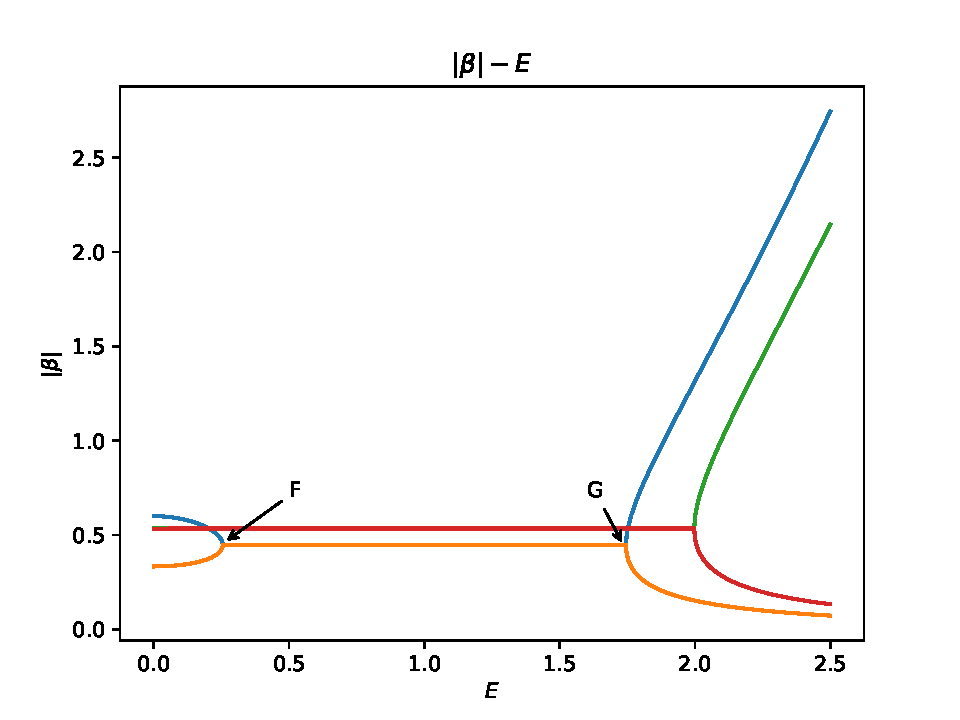
\includegraphics[width=4in]{Figure_5.pdf}
    \caption{$|t_1|=1$和$t_1=1.2$在$t_2=1,\gamma=4/3$条件下解的分布}
\end{figure}
\begin{lstlisting}
    mport numpy as np
    import matplotlib.pyplot as plt
    from numpy.random import gamma
    t1=1
    gamma=4/3
    t2=1
    def beta(E,n):
        a=[(t1+gamma/2)*t2,t1**2-gamma**2/4+t2**2-E**2,(t1-gamma/2)*t2]
        result=np.roots(a)
        return abs(result[n])
    energy=np.linspace(0,2.5,10000)
    for n in [0,1]:
        ybeta=[beta(x,n) for x in energy]
       plt.plot(energy,ybeta)

    t1=1.2
    gamma=4/3
    t2=1
    def beta(E,n):
        a=[(t1+gamma/2)*t2,t1**2-gamma**2/4+t2**2-E**2,(t1-gamma/2)*t2]
        result=np.roots(a)
        return abs(result[n])
    energy=np.linspace(0,2.5,10000)
    for n in [0,1]:
        ybeta=[beta(x,n) for x in energy]
        plt.title(r'$|\beta|-E$') 
        plt.xlabel(r"$E$") 
        plt.ylabel(r"$|\beta|$")
        plt.plot(energy,ybeta)
        plt.annotate("F", (0.258,0.458), xycoords='data',
                xytext=(0.5,0.7), 
                arrowprops=dict(arrowstyle='->')) 
        plt.annotate("G", (1.738,0.442), xycoords='data',
                xytext=(1.6,0.7), 
                arrowprops=dict(arrowstyle='->')) 
    plt.show()
\end{lstlisting}
对于这个参数集能谱是实的,因此$E$没有虚部是必须的(实际上依赖于$PT$对称性)。所期待的$|\beta_1|=|\beta_2|=r$关系被发现在上图中端,这与体态能谱相联系。当$t_1$从1增加时,$F$点向左移动,最终撞到$|\beta|$轴上。显然的,这发生在$|\beta_1^{E\to0}|=|\beta_2^{E\to0}|=r$时。把零能对应的$\beta$解带进去得到
\begin{equation}
    |\frac{t_1-\gamma/2}{t_2}|=|\frac{t_2}{t_1+\gamma/2}|\Rightarrow t_2^2=|t_1^2-\gamma^2/4|\Rightarrow \begin{cases}
        t_1=\pm\sqrt{t_2^2+\gamma^2/4}&(|t_1|>|\gamma/2|)\\
        t_1=\pm\sqrt{-t_2^2+\gamma^2/4}&(|t_1|<|\gamma/2|)
    \end{cases}
\end{equation}
在这些点处,开边界连续谱达到零能,能发生拓扑相变。

类似的方式计算相变点是通过计算开边界能谱。对方程
\begin{equation}
    \left[\left(t_1-\frac{\gamma}{2}\right)+t_2\beta\right]\left[\left(t_1+\frac{\gamma}{2}\right)+t_2\beta^{-1}\right]=E^2
\end{equation}
做一个替换$\beta=r e^{ik},a=1,k\in[0,2\pi]$
\begin{equation}
    \begin{split}
        E^2(k)&=\left[(t_1-\frac{\gamma}{2})+t_2 r e^{ik}\right]\left[(t_1+\frac{\gamma}{2})+t_2 r^{-1}e^{-ik}\right]\\
        &=t_1^2+t_2^2-\frac{\gamma^2}{4}+t_2re^{ik}(t_1+\frac{\gamma}{2})+(t_1-\frac{\gamma}{2})t_2r^{-1}e^{-ik}\\
        &=t_1^2+t_2^2-\frac{\gamma^2}{4}+t_2\sqrt{|t_1^2-\frac{\gamma^2}{4}|}\mathrm{sgn}(t_1+\frac{\gamma}{2})e^{ik}+t_2\sqrt{|t_1^2-\frac{\gamma^2}{4}|}\mathrm{sgn}(t_1-\frac{\gamma}{2})e^{-ik}
    \end{split}
\end{equation}
当$\gamma=0$时,回到SSH模型。当$|t_1|>|\gamma/2|$时,能谱是实的:
\begin{equation}
    E^2(k)=t_1^2+t_2^2-\gamma/4\pm 2t_2\sqrt{t_1^2-\gamma^2/4}\cos k
\end{equation}
能隙闭合条件为$t_1^2+t_2^2-\gamma^2/4=0$或者$\sqrt{t_1^2-\gamma^2/4}=t_2$,这与相变条件一致。

在继续之前,我们先讨论一下寻找零模的标准方法中的一个微妙问题。为具体起见,我们考虑本模型,关注长链左端零模态。我们可以看到$|\psi^{zero}\rangle$有$(\psi_{n,A}^{zero},\psi_{n,B}^{zero})=(\beta_1^{E\to 0})^n(1,0)$出现一个零模本征态。按照标准方法,归一化条件要求$|\beta_1^{E\to 0}|<1$,并且相变点满足$|\beta_1^{E\to 0}|=1$,这个条件可以推出$t_1=t_2+\frac{\gamma}{2}$作为相变点,与$H(k)$对应的能隙关闭条件一致。这种明显并且具有误导性的一致性在以前的非厄米模型的研究中隐藏了真正的相变点和拓扑不变量。隐含的假设是体本征态是广义的布洛赫波,在相变点处$|\beta|=1$转化到体本征态。事实上,体本征态有$|\beta|=r$;因此,真正转化到体态的条件是
\begin{equation}
    |\beta_1^{E\to0}|=r
\end{equation}
这正确的得到了$t_1=\sqrt{t_2^2+(\gamma/2)^2}$. 这是非布洛赫体边界对应的一种表现。
\section{非布洛赫拓扑不变量}
如果我们能找到决定边缘模的体拓扑不变量,那么体边对应关系就会被满足。以前从$H(k)$为起点构建的理论应该在非厄米趋肤效应上修改。通常的布洛赫波承载一个纯粹的相因子$e^{ik}$,现在这个作用由$\beta$来承担。除了相因子,$\beta$的模一般满足$|\beta|\neq1$. 因此我们从通过替换$e^{ik}\rightarrow\beta,e^{-ik}\rightarrow\beta^{-1}$获得的非厄米哈密顿开始
\begin{equation}
    H(\beta)=\left(t_1-\frac{\gamma}{2}+\beta t_2\right)\sigma_-+\left(t_1+\frac{\gamma}{2}+\beta^{-1}t_2\right)\sigma_+
\end{equation}
\begin{equation}
    \sigma_-=\begin{pmatrix}
        0&0\\
        1&0
    \end{pmatrix},\quad\sigma_+=\begin{pmatrix}
        0&1\\
        0&0
    \end{pmatrix}
\end{equation}
为了简单起见,我们令$t_3=0$. 正如在截断解和一般解里所说,$\beta$的取值是在一个非单位圆周$|\beta|=r$上。换句话说,$k$获得了一个相位$-i\ln r$. 值得注意的是,上节末尾的开边界能谱是由$H(\beta)$给出,而不是由$H(k)$给出。

左手本征矢量和右手本征矢量被定义为:
\begin{equation}
    H(\beta)|u_R\rangle=E(\beta)|u_R(\beta)\rangle,\quad H^\dagger(\beta)|u_L(\beta)\rangle=E^*(\beta)|u_L(\beta)\rangle
\end{equation}
子格对称性要求,$\sigma_z^{-1}H(\beta)\sigma_z=-H(\beta)$. 所以有
\begin{equation}
    \begin{split}
        &\sigma_z^{-1}H(\beta)\sigma_z|u_R(\beta)\rangle=-H(\beta)|u_R(\beta)\rangle=-E(\beta)|u_R(\beta)\rangle\Rightarrow H(\beta)|\tilde{u}_R(\beta)\rangle=-E|\tilde{u}_R(\beta)\rangle\\
        &\sigma_z^{-1}H^\dagger(\beta)\sigma_z|u_L(\beta)\rangle=-H^\dagger(\beta)|u_L(\beta)\rangle=-E^*(\beta)|u_L(\beta)\rangle\Rightarrow H^\dagger(\beta)|\tilde{u}_L(\beta)\rangle=-E^*(\beta)|\tilde{u}_L(\beta)\rangle
    \end{split}
\end{equation}
其中$|\tilde{u}_R\rangle=\sigma_z|u_R\rangle,|\tilde{u}_L\rangle=\sigma_z|u_L\rangle$,分别对应本征值$-E$和$-E^*$. 实际上,矩阵可以被对角化为$H(\beta)=TJT^{-1}$,其中$J=\begin{pmatrix}
    E\\
    &-E
\end{pmatrix}$, $T$和$(T^{-1})^\dagger$的每一列分别是右手/左手本征矢量:
\begin{equation}
    T=\begin{pmatrix}
        |u_R\rangle&|\tilde{u}_R\rangle
    \end{pmatrix},\quad T^{-1}=\begin{pmatrix}
        \langle u_L|&\langle\tilde{u}_L|
    \end{pmatrix}
\end{equation}
归一化正交条件为
\begin{equation}
    \langle u_L|u_R\rangle=\langle\tilde{u}_L|\tilde{u}_R\rangle=1
\end{equation}
\begin{equation}
    \langle u_L|\tilde{u}_R\rangle=\langle\tilde{u}_L|u_R\rangle=0
\end{equation}
利用$Q$矩阵进行推广,我们定义
\begin{equation}
    Q(\beta)=|\tilde{u}_R(\beta)\rangle\langle\tilde{u}_L(\beta)|-|u_R(\beta)\rangle\langle u_L(\beta)|
\end{equation}
由于子格对称性
\begin{equation}
    \sigma_z^{-1}Q\sigma_z=\sigma_z|\tilde{u}_R(\beta)\rangle\langle\tilde{u}_L(\beta)|\sigma_z-\sigma_z|u_R(\beta)\rangle\langle u_L(\beta)|\sigma_z=|u_R(\beta)\rangle\langle u_L(\beta)|-|\tilde{u}_R(\beta)\rangle\langle \tilde{u}_L(\beta)|=-Q
\end{equation}
也就是说$Q=\begin{pmatrix}
    &q\\
    q^{-1}&
\end{pmatrix}$. 我们现在引入非布洛赫缠绕数
\begin{equation}
    W=\frac{i}{2\pi}\int_{C_\beta}q^{-1}dq
\end{equation}
为了计算出缠绕数,我们可以假设$|u_R\rangle=\begin{pmatrix}
    \alpha_1\\
    \alpha_2
\end{pmatrix},|u_L\rangle=\begin{pmatrix}
    \eta_1\\
    \eta_2
\end{pmatrix}$,能量本征方程为
\begin{equation}
    \begin{split}
        H(\beta)\begin{pmatrix}
            \alpha_1\\
            \alpha_2
        \end{pmatrix}=E(\beta)\begin{pmatrix}
            \alpha_1\\
            \alpha_2
        \end{pmatrix}\\
        H^\dagger(\beta)\begin{pmatrix}
            \eta_1\\
            \eta_2
        \end{pmatrix}=E^*(\beta)\begin{pmatrix}
            \eta_1\\
            \eta_2
        \end{pmatrix}
    \end{split}
\end{equation}
其中$H(\beta)=\begin{pmatrix}
    0&d_+\\
    d_-&0
\end{pmatrix}$. 可以计算出能量$E,E^*$对应本征矢量分别为
\begin{equation}
    |u_R\rangle=\alpha_2\begin{pmatrix}
        \frac{d_+}{E}\\
        1
    \end{pmatrix},\quad |u_L\rangle=\eta_2\begin{pmatrix}
        \frac{d_-^*}{E^*}\\
        1
    \end{pmatrix}
\end{equation}
由于子格对称性,可以得到$-E,-E^*$对应的本征态为
\begin{equation}
    |\tilde{u}_R\rangle=\sigma_z|u_R\rangle=\alpha_2\begin{pmatrix}
        \frac{d_+}{E}\\
        -1
    \end{pmatrix},\quad |\tilde{u}_L\rangle=\eta_2\begin{pmatrix}
        \frac{d_-}{E^*}\\
        -1
    \end{pmatrix}
\end{equation}
其中$E=\pm\sqrt{d_+d_-}$. 利用归一化条件$\langle u_L|u_R\rangle=1$可以得到
\begin{equation}
    \langle u_L|u_R\rangle=\alpha_2\eta_2^*(\frac{d_+d_-}{E^2}+1)=2\alpha_2\eta_2^*=1\Rightarrow \alpha_2\eta_2^*=\frac{1}{2}
\end{equation}
所以可以计算出$Q$矩阵
\begin{equation}
    \begin{split}
        Q(\beta)&=|\tilde{u}_R\rangle\langle\tilde{u}_L|-|u_R\rangle\langle u_L|\\
        &=\alpha_2\eta_2^*\begin{pmatrix}
            \frac{d_+}{E}\\
            -1
        \end{pmatrix}\begin{pmatrix}
            \frac{d_-}{E}&-1
        \end{pmatrix}-\alpha_2\eta_2^*\begin{pmatrix}
            \frac{d_+}{E}\\
            1
        \end{pmatrix}\begin{pmatrix}
            \frac{d_-}{E}&1
        \end{pmatrix}\\
        &=\frac{1}{2}\left(\begin{pmatrix}
            \frac{d_+d_-}{E}&-\frac{d_+}{E}\\
            -\frac{d_-}{E}&1
        \end{pmatrix}-\begin{pmatrix}
            \frac{d_+d_-}{E}&\frac{d_+}{E}\\
            \frac{d_-}{E}&1
        \end{pmatrix}\right)\\
        &=\begin{pmatrix}
            &-\sqrt{\frac{d_+}{d_-}}\\
            -\sqrt{\frac{d_-}{d_+}}&
        \end{pmatrix}
    \end{split}
\end{equation}
我们得到$q=-\sqrt{\frac{d_+}{d_-}}$. 最终计算出缠绕数为
\begin{equation}
    \begin{split}
        \frac{i}{2\pi}\int_{C_\beta}q^{-1}\mathrm{d}q&=\frac{i}{2\pi}\int_{C_\beta}\mathrm{d}\ln q\\
        &=\frac{i}{2\pi}\int_{C_\beta}\mathrm{d}\left(\ln |q|+i\arg q\right)\\
        &=-\frac{1}{2\pi}\arg q|_{C_\beta}=\left.-\frac{1}{2\pi}\arg\sqrt{\frac{d_+}{d_-}}\right|_{C_\beta}\\
        &=\left.-\frac{1}{4\pi}(\arg d_+-\arg d_-)\right|_{C_\beta}
    \end{split}
\end{equation}
其中$C_\beta$是布里渊区$|\beta|=r=\sqrt{|\frac{t_1-\gamma/2}{t_1+\gamma/2}|}$
\begin{figure}[h]
    \centering
    \animategraphics[width=3in,autoplay=True]{24}{dcomplex/}{1}{300}
    \caption{$t_1$从$-3$到$3$变化过程中$d$在复空间路径的变化}
\end{figure}
\begin{figure}[h]
    \centering
    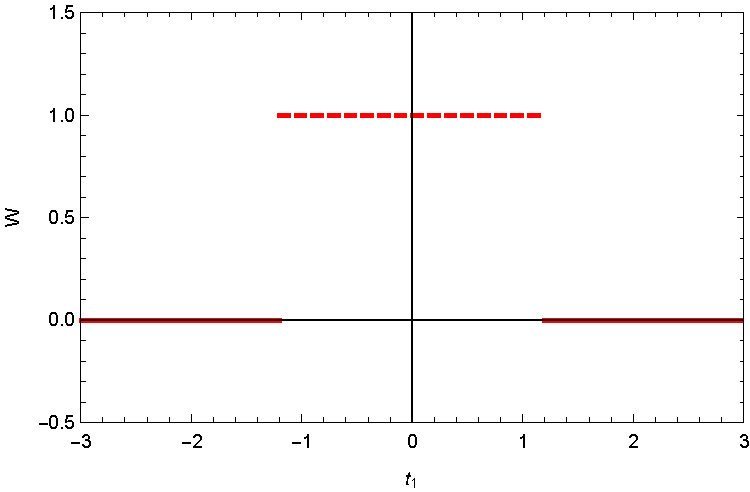
\includegraphics[width=3in]{windingnumber.pdf}
    \caption{缠绕数随$t_1$的变化}
\end{figure}
严格的来说,上面的计算是在广义的布里渊区$C_\beta$上计算的。值得注意的是如果$C_\beta$正好是一个单位圆,传统用$H(k)$来计算有时候有可能产生一个正确的相图

$t_3=0$的数值结果如上图所示,这与解析结果一致。数值上来说,$2W$描述了Robust零模在左端或者右端的总数。例如对于上面描述的SSH模型,在$t\in[-\sqrt{t_2^2+(\frac{\gamma}{2})^2},\sqrt{t_2^2+(\frac{\gamma}{2})^2}]$有两个零模,在这个范围以外没有零模。在$t_1\in[t_2-\gamma/2,\sqrt{t_2^2+(\gamma/2)^2}]$,两个零模都在左端。在$t_2\in[-t_2+\gamma/2,t_2-\gamma/2]$,两个零模分别一个在左边一个在右边。在$t_1\in[-\sqrt{t_2^2+(\gamma/2)^2}]$,两个零模都在右边。因此$H(k)$能带闭合点$\pm(t_2-\gamma/2)$是零模交换左右的点,总的模数守恒。事实上,可以看到$|\beta_{1,2}^{E\to0}|=1$在$\pm(t_2-\gamma/2)$,渗透到体态中。

最后我们强调缠绕数方程可以推广到多带系统中。每一对能带$l$占据一个$C_{\beta}^{l}$曲线,并且$Q$矩阵变成$Q^{(l)}$,每一个$Q^{(l)}$定义了一个缠绕数$W^{(l)}$。拓扑不变量是$W=\sum_lW^{(l)}$









\end{document}